\documentclass{beamer}

\usepackage[utf8]{inputenc}
\usepackage[T1]{fontenc}
\usepackage[english]{babel}
\usepackage{tikz}
\usepackage{algorithm}
\usepackage{algorithmicx}
\usepackage{algpseudocode}
\usepackage{amsmath}
\usepackage{mathtools}

\usetheme{Madrid}

\title{Dynamical Processes : Presentation}
\subtitle{Anomalous versus Slowed-Down Brownian Diffusion
in the Ligand-Binding Equilibrium \\ H. Soula et. al.}
\author{Marc Heinrich \\ Clément Henin}
\date\today

\AtBeginSection[]{
  \stepcounter{subsection}
  \begin{frame}
  \vfill
  \centering
  \begin{beamercolorbox}[sep=8pt,center,shadow=true,rounded=true]{title}
    \usebeamerfont{title}\insertsectionhead\par%
  \end{beamercolorbox}
  \vfill
  \end{frame}
}

\begin{document}

\begin{frame}
\maketitle
\end{frame}

\begin{frame}
\frametitle{Introduction}
%Justification of the study: 
	% Anomalous diffusion in molecules
	
\begin{itemize}
\itemsep2em
\item Study of protein motion in cells show anomalous behaviour
\item At long times, it converges to Brownian motion with reduced diffusion coefficient
\item Study models for the movement of proteins in particles
\end{itemize}
\end{frame}

\begin{frame}{Ligand Binding reaction}
\begin{block}{Equation}

\begin{align*}
\mathrm{L+R} \xrightleftharpoons[k_{on}]{k_{off}} \mathrm{C}
\end{align*}
\end{block}

\pause

\begin{itemize}
\itemsep1em
\item Mass action law equation: $\frac{d[C]}{dt} = - k_{off}[C] + k_{on}[L][R] $ 
\pause
\item We work in the case $[L] \gg [R]$
\item Mass action law solution converges to $[C]_{eq} = \frac{[L]_0 [R]_0}{[L]_0 + \frac{k_{off}}{k_{on}}}$ 
\end{itemize}
\end{frame}

\begin{frame}{Anomalous diffusion}

\begin{figure}
%TODO : put here the image from 
\caption{Anomalous diffusion for short time, converges to Brownian motion at long times}
\end{figure}

\end{frame}


\section{Three Models}

\begin{frame}
Présentation de la grille et des movings particles
+ 
Présentation du patch (avec un petit schéma)
\begin{block}{}
\begin{itemize}
\itemsep1em
\item Particles moving on a $2D$ grid
\item At each time step a particle has a probability of leaving $p_{move}(i,j)$
\item $2$ zones: central patch area, and the rest of the grid
\item when L and R have the same coordinates then $p_{on}$ to react
\item C have $p_{off}$ to decompose in L and R
\end{itemize}
\end{block}

\end{frame}

\begin{frame}{Brownian motion with two diffusion coefficients}
\begin{block}{Model}
\begin{itemize}
\itemsep1em
\item Diffusion coefficients: $D_{patch}$, $D_{ext}$
\end{itemize}
\end{block}

\begin{align*}
p_{move} = \frac{4 \Delta t}{(\Delta x)^2} D(i,j)
\end{align*}

\end{frame}

\begin{frame}{Brownian motion with immobile obstacles}
% Put the definition here
% General behaviour : brownian motion at small and large time scales
\begin{block}{Model}
\begin{itemize}
\itemsep1em
\item Obstacles in the patch with probability $\rho$
\item exclude the lattice site they occupy
\item when particule hits obstacle it comes back to its origin
\end{itemize}
\end{block}


Percolation threshold : $\rho \approx 0.407253949$


\end{frame}

\begin{frame}
\begin{center}
\Huge \color{blue} Example
\end{center}
\end{frame}

\begin{frame}{CTRW}
% Definition + general behaviour (mean square deviation)
\begin{block}{Model}
Residence time of a particle in the grid given by power law with cut-off: 
$$ \phi(\tau) \propto \alpha \tau^{-(1+\alpha)} \mathbf{1}_{\tau < \tau_c}$$
\end{block}
%TODO : draw a graph of the distribution?
%Put figure 1 B here

\end{frame}


\section{Simulations}

\begin{frame}{Parameters}
$$
\begin{array}{|c|c|}
\hline
Parameter & value \\
\hline
\Delta t & 1 \\
\Delta x & 2 \\
\text{grid size} & 800 \times 800 \\
n_A & 100 \\
n_B & 4500 \\
\hline
D_{patch} & [0.01, 1] \\
D_{ext} & 1 \\
\rho & [0, 0.4] \\
\hline
\alpha & [0,1] \\
\tau_c & [10^1, 10^6] \\
\hline
\end{array}
$$
\end{frame}

\begin{frame}{Time evolution of C: Brownian model}
%Time evolution of number of C for the brownian model
% For several values of D
%Value at equilibrium does not depend on D

\begin{figure}
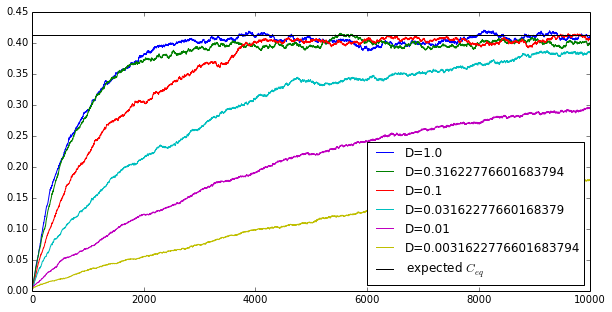
\includegraphics[width=\textwidth]{C_Dvar}
\caption{Time evolution of the number of $C$ for different value of $D$. Patch size$=100\%$. Equilibrium is independant of $D$}
\end{figure}
\end{frame}

\begin{frame}
{Time evolution of C: Brownian model}
\begin{figure}
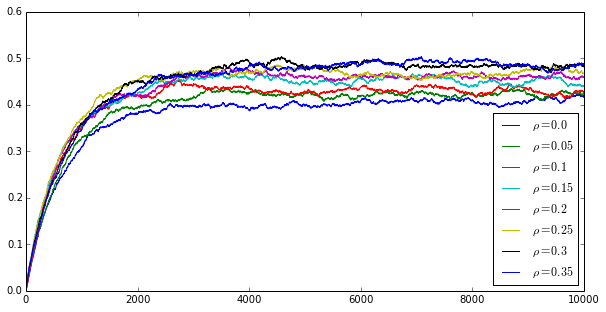
\includegraphics[width=\textwidth]{C_rhovar}
\caption{Time evolution of the number of $C$ for different value of $\rho$. Patch size$=100\%$}
\end{figure}
\end{frame}


\begin{frame}
\begin{figure}
%Figure for browninan motion with obstacles
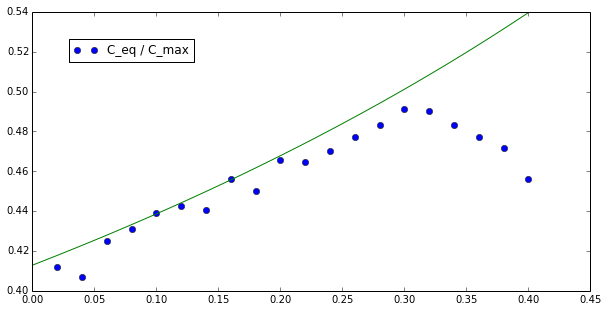
\includegraphics[width=\textwidth]{Ceq_rhovar}
\caption{Equilibrium value as a function of $\rho$}
\end{figure}
\end{frame}

\begin{frame}
%Show the four graphics from the article
\begin{figure}
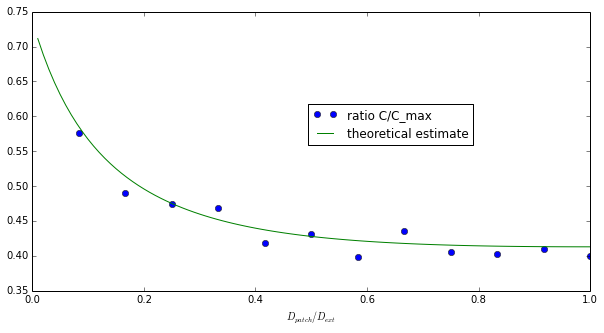
\includegraphics[width=.5\textwidth]{Ceq_D0var}
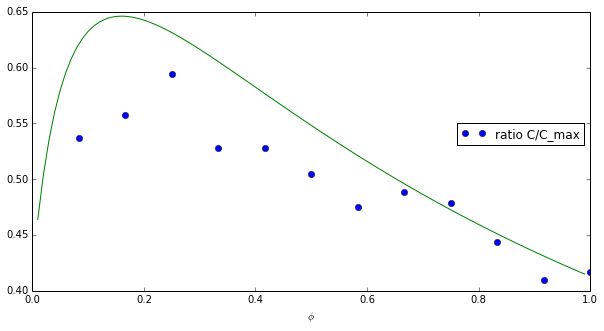
\includegraphics[width=.5\textwidth]{Ceq_phivar}
\caption{Comparing theoretical estimate with values from the experiments}
\end{figure}
\end{frame}

\begin{frame}
\begin{figure}
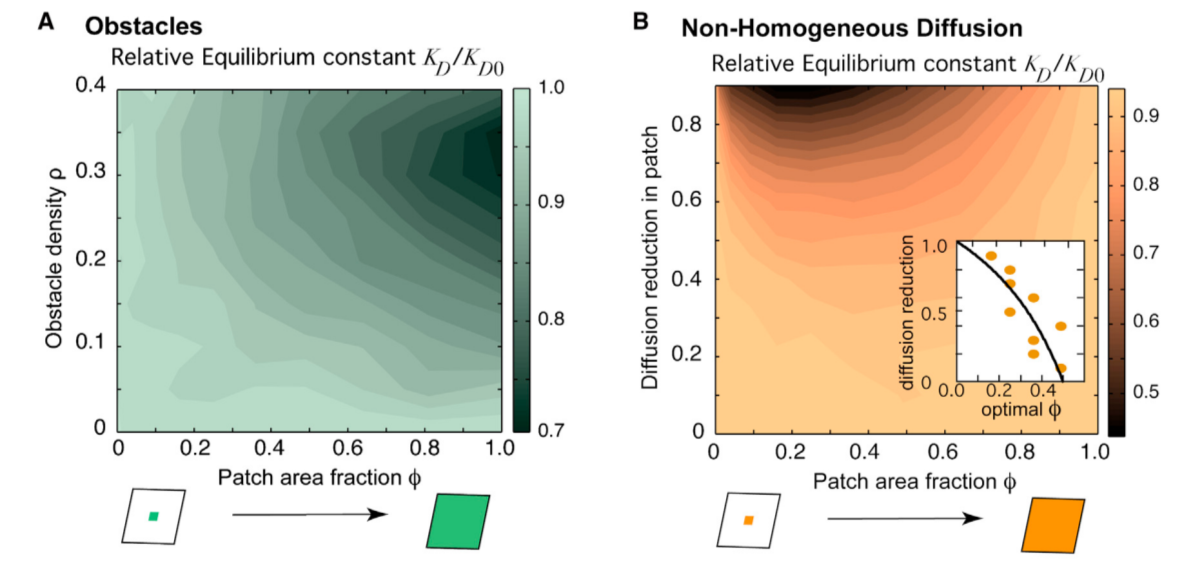
\includegraphics[width=\textwidth]{2Dplots}
\caption{Equilibrium constant depending on the type of patch, and its size}
\end{figure}
\end{frame}


%TODO : eventually put here other plots for the CTRW model

\begin{frame}{Time evolution of C: CTRW model}
\begin{figure}
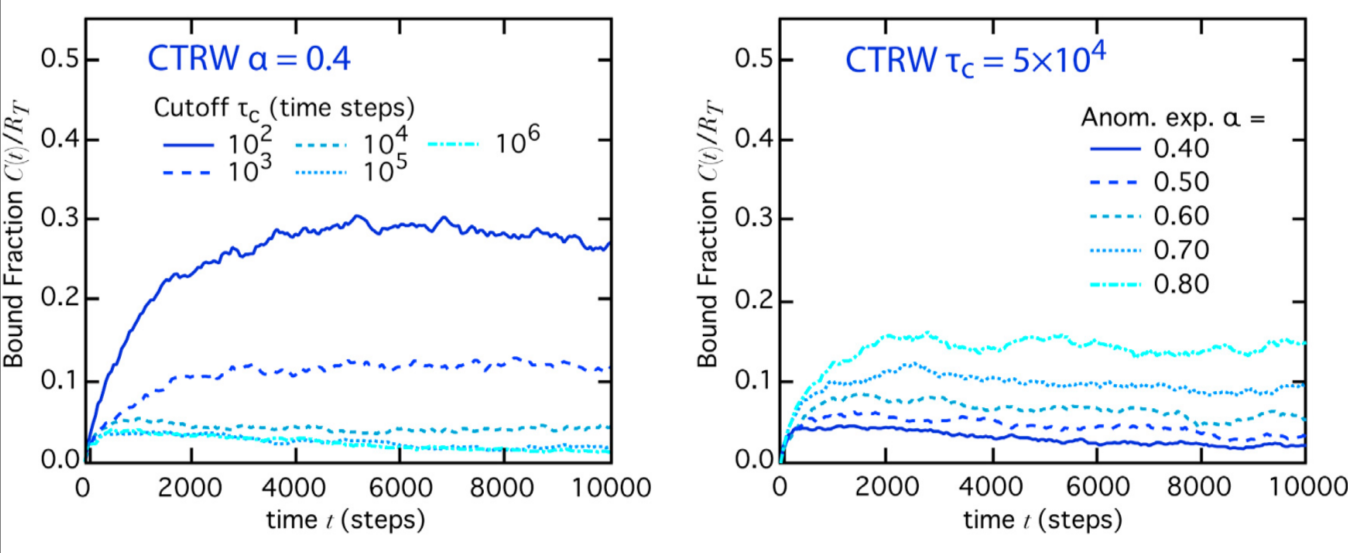
\includegraphics[width=\textwidth]{CTRW}
\caption{Time evolution of the number of $C$ for different values of $\tau_c$ and $\alpha$}
\end{figure}
\end{frame}


\begin{frame}{Conclusion}
% Study of different diffusion model
% Attempt to model anomalous diffusion in cells
% Study the influence of this anomalous diffusion on reactions, and equilibrium of these reactions

\begin{itemize}
\itemsep2em
\item Study different diffusion models
\item Attempt to model influence of anomalous diffusion on reaction
\item Influence of the model on equilibrium
\end{itemize}
\end{frame}

\begin{frame}
\begin{center}
\Huge \color{blue} Thank you!
\end{center}
\end{frame}

\end{document}